\subsection{Objetivo}

	En esta primera etapa se busca calcular el volumen de la sala, y planificar el esquema de planta de la misma. En concreto, se debe:

	\begin{itemize}
		\item Especificar la altura elegida del recinto;
		\item Especificar la capacidad de la sala (cantidad de butacas que se instalarán);
		\item Realizar un esquema de planta: ubicación de butacas, oradores, puertas, pasillos, etc;
		\item Indicar las dimensiones más relevantes: pasillos, puertas, espacio para oradores, butacas, separación entre butacas, etc.
	\end{itemize}

\subsection{Importancia de las dimensiones del recinto}

Un factor importante que afecta el comportamiento de los recintos son sus \textsc{modos de resonancia}:

\begin{itemize}
	\item Cuando el sonido se refleja entre dos superficies paralelas, se producen interferencias constructivas y destructivas, dando lugar a la formación de ondas estacionarias o \textit{modos propios de la sala};
	\item Es una característica propia de cada sala y el efecto que produce se denomina \textit{coloración}. Es más común en recintos pequeños, como los estudios de grabación, por ejemplo.
\end{itemize}

Un \textit{modo propio} es una onda estacionaria generada en el interior de una sala. Se producen por la interacción entre las ondas incidentes y reflejadas dentro del recinto. Cada modo está asociado a una frecuencia (frecuencia propia).\\

Si la distancia entre dos superficies paralelas de una sala es igual a media longitud de onda (d = $\lambda/2)$, se generará una onda que permanecerá estacionaria reflejándose entre las dos superficies paralelas, perdiendo paulatinamente energía acústica. Estos refuerzos ocurrirán fundamentalmente para tres frecuencias básicas correlacionadas con las dimensiones del recinto (largo, ancho y altura) y para sus múltiplos.\\

Según la cantidad de superficies que intervengan, los modos podrán ser \textsc{axiales} (se establecen entre dos superficies), \textsc{tangenciales} (entre cuatro superficies) u \textsc{oblicuos} (entre las seis superficies del recinto).\\

El cálculo de frecuencias de modos de resonancia o modos propios se realiza de acuerdo a la siguiente expresión:

\begin{equation}
	f_{modos} = \frac{c}{2}\,\sqrt{\left(\frac{p}{L} \right)^2 + \left(\frac{q}{W} \right)^2 + \left(\frac{r}{H} \right)^2},\quad \forall\, p,q,r \,\in \mathbb{Z}
\end{equation}

Donde:

\begin{itemize}
	\item $f_m$: frecuencia del modo de resonancia;
	\item $c$: velocidad del sonido, en m/s;
	\item $p,\,,\,r$: números enteros que denotan el número de medias longitudes de onda en las 3 direcciones (0, 1, 2,...);
	\item $L,\,W,\,H$: las dimensiones del recinto, en m.
\end{itemize}

Según el valor que tomen p, q y r en la expresión anterior:

\begin{itemize}
	\item Si uno es distinto de cero, son modos \textsc{axiales};
	\item Si dos son distintos de cero, son modos \textsc{tangenciales};
	\item Si tres son distintos de cero, son modos \textsc{oblicuos}.
\end{itemize}

\subsection{Aplicación del criterio de Bonello}

Bonello contempla todos los modos presentes, fijando el análisis sobre la base de porcentajes de la frecuencia modal y no a distancias fijas.\\ 

Primero, se calculan todas las frecuencias de modos propios del recinto que estén por debajo de la \textsc{frecuencia de Schroeder}, que está dada por la siguiente expresión:

\begin{equation}
	f_s = 1893\,\sqrt{\frac{TR}{V}}
\end{equation}

Luego, se divide el espectro en tercios de octava hasta la $f_s$ obtenida, pues el análisis por tercios satisface a la discriminación de frecuencias del oído.\\

El último paso es calcular y graficar la \textit{densidad de modos} (cantidad de modos por cada tercio de octava).\\

Finalmente, para decidir si cumple con el Criterio de Bonello, se debe cumplir que:

\begin{enumerate}
	\item La curva de densidad de modos debe ser monótonamente creciente, o a lo sumo tener la misma cantidad de modos en dos tercios de octava sucesivos;
	\item No deben existir modos dobles y, si los hubiera, se los tolera en tercios de octava con densidad de modos mayor que cinco.
\end{enumerate}


%% Valor aceptable en ambientes desocupados (sin personas) / criterio NC recomendado para sala de conferencias: NC25-30.

\subsection{Cálculos}

Para aplicar el criterio, se acude a alguna herramienta online de cálculo; en este caso, se usó \texttt{amroc: the room mode calculator}\footnote{https://amcoustics.com/tools/amroc}. Es muy útil para ver cómo varía la distribución de los modos de acuerdo a las dimensiones del salón.\\

\HgraficarPNG{0.45}{amroc_parámetros.png}{Parámetros finales usados para aplicar el criterio de Bonello.}{amroc_parámetros}

Primero se fijaron las dimensiones de ancho y largo del recinto, que son dato; luego, de indicó la norma correspondiente para tener el \texttt{RT60} adecuado (en este caso, se sabe que es una sala destinada a la palabra, por lo que se seleccionó \textit{Speech}). La dimensión restante, que es la altura, se fue variando entre los límites de lo que se considera una altura sensata para una sala de conferencias, en cuanto a términos de arquitectura. Luego de consultar varias fuentes y de dimensionar el recinto con una herramienta CAD, se llegó a un valor de altura \texttt{H = 4.9m}. Si bien, una altura más baja podría ser considerada un poco más apropiada visualmente, esta altura elegida cumple perfectamente con el criterio de Bonello, y tampoco es tan grande como para ser considerada desproporcionada.

Con la altura elegida, el gráfico de Bonello que muestra la herramienta se ve así:

\HgraficarPNG{0.7}{amroc_bonello.png}{Gráfico de la cantidad de modos por tercio de octava que provee la herramienta.}{amroc_bonello}

A partir de este gráfico, se puede concluir en que el criterio se cumple para este valor de altura elegido, ya que es monótonamente creciente (sólo hay dos bandas de octava con la misma cantidad de modos, pero cumplen con el criterio por ser consecutivas).

\HgraficarPNG{0.55}{amroc_adicional.png}{Información adicional que provee la herramienta.}{amroc_adicional}

En la Figura \ref{amroc_adicional}, se puede ver que gracias a esta herramienta, también se obtiene el cálculo del volumen y la superficie del recinto, así como el valor de la frecuencia de Schroeder y la distancia crítica (que sirve para el análisis de la segunda etapa).\\

La frecuencia de Schroeder se puede calcular como:

\begin{equation}
	f_s = 1893\,\sqrt{\frac{TR}{V}} = 1893\,\sqrt{\frac{0.75\,s}{438.35\,m^3}} \approx 78 Hz
\end{equation}

	A diferencia del valor calculado, la herramienta provee un valor de $f_s =$ \SI{83}{\Hz}, que resulta de calcular la expresión de arriba con un factor de $2000$ en vez de $1893$; esta aproximación se suele utilizar.\\

	Recortando entonces el rango de frecuencias de interés, se calcularon un total de 45 modos, que se verán detallados en la siguiente Tabla (repartida en las Figuras \ref{amroc_tabla_1}, \ref{amroc_tabla_2}). Para cada modo, se indica la frecuencia eel mismo, si es axial, tangencial u oblicuo, y la combinación de los parámetros p, q, r que logran dicho modo:
	
	\begin{figure}[H]
		\centering
		\begin{subfigure}{.5\textwidth}
  			\centering
  			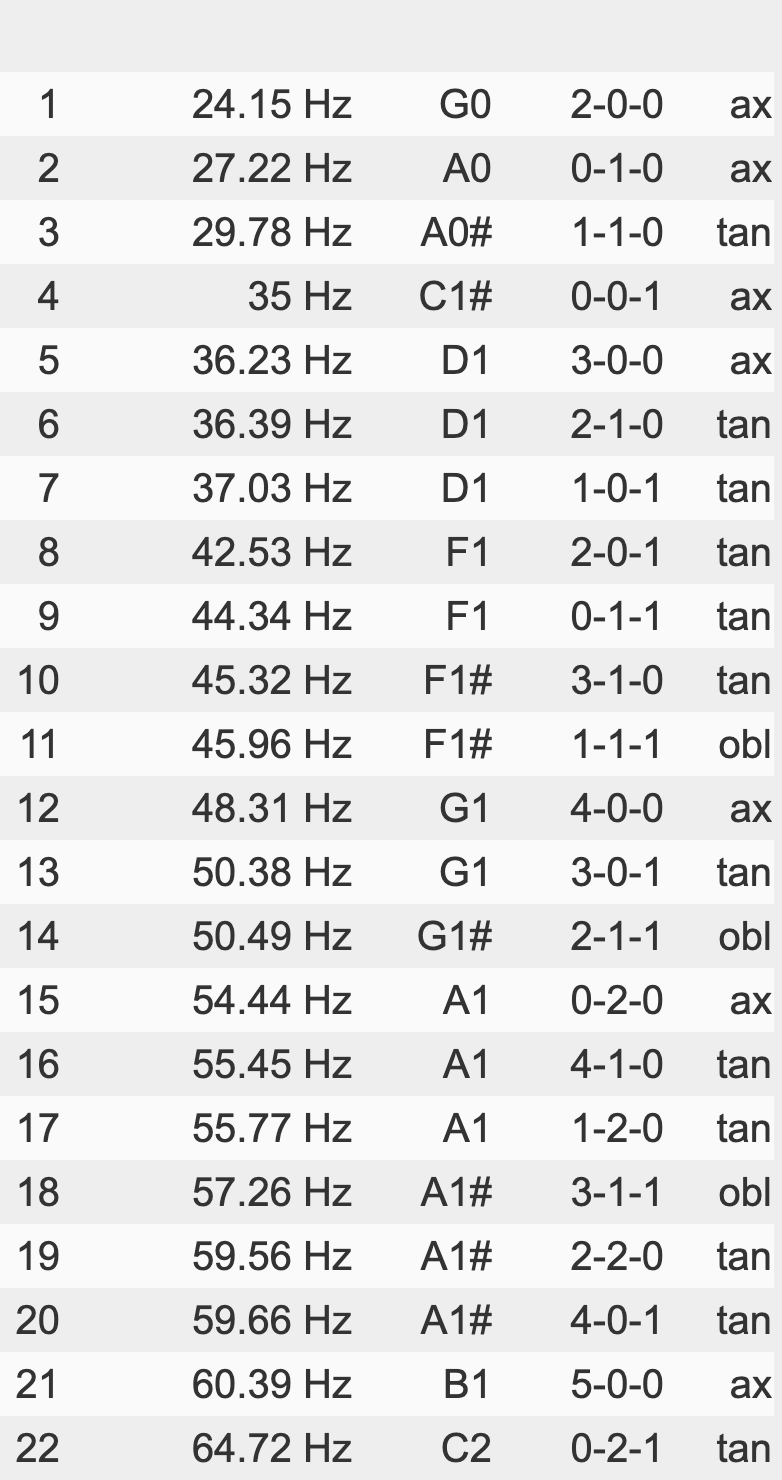
\includegraphics[width=0.8\linewidth]{amroc_tabla_1.png}
  			\caption{Rango de frecuencias 24.1-65.4Hz}
  			\label{amroc_tabla_1}
		\end{subfigure}%
		\begin{subfigure}{.5\textwidth}
  			\centering
  			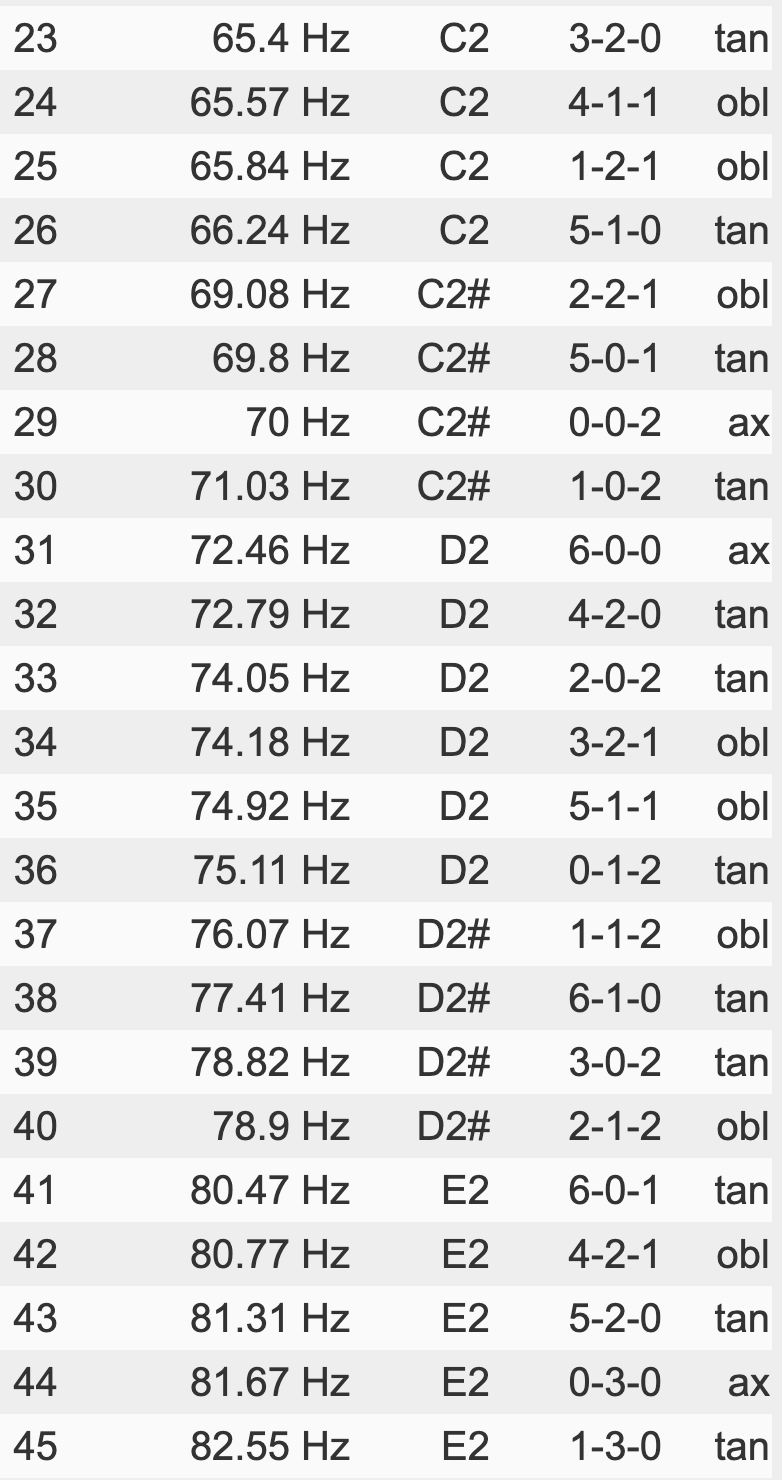
\includegraphics[width=0.8\linewidth]{amroc_tabla_2.png}
  			\caption{Rango de frecuencias 65.5-82.55Hz.}
  			\label{amroc_tabla_2}
		\end{subfigure}
		\caption{Tabla con la información detallada de todos los modos analizados entre las frecuencias de interés.}
		\label{amroc_tablas}
	\end{figure}

En estas tablas, se puede comprobar que se cumple con el segundo criterio de Bonello, ya que no existen modos iguales.\\

A partir de los datos relevados de estas tablas, se graficó la cantidad de modos por tercio de octava, para comprobar que resultara como en la simulación, y se obtuvo lo siguiente:

\HgraficarPNG{0.4}{curva_bonello.png}{Esquema de la planta que será utilizada como una sala de conferencias.}{curva_bonello}

Se pueden notar algunas diferencias con la curva que provee la herramienta, pero lo importante es que sigue cumpliendo con el criterio de Bonello: es monótonamente creciente (cumple con el primer criterio de Bonello). Las diferencias se dan por la cantidad de modos que considera la herramienta: toma 29 modos, mientras que en mi caso tomo los 45 modos que me provee la tabla.\\

Luego de estos cálculos, se presentan una tabla con los parámetros de interés para el recinto:

		\begin{table}[h!]
			\centering
			\begin{tabular}{cc}
			\toprule
			\textbf{Largo} & \textbf{\SI{14.2}{\m}}\\
			\midrule
			\textbf{Ancho} & \textbf{\SI{6.3}{\m}}\\
			\midrule
			\textbf{Alto} & \textbf{\SI{4.9}{\m}}\\
			\midrule
			\textbf{Volumen} & \textbf{\SI{438.354}{\cubic\m}}\\
			\midrule
			\textbf{Superficie} & \textbf{\SI{379.82}{\square\m}}\\
			\midrule
			\textbf{Frecuencia de Schröder} & \textbf{\SI{83}{\Hz}}\\
			\midrule
			\textbf{Tiempo de reverberación} & \textbf{\SI{0.75}{\s}}\\
			\midrule
			\textbf{Distancia crítica} & \textbf{\SI{1.38}{\m}}\\
			\bottomrule
			\end{tabular}
		\end{table}

Para entender mejor las dimensiones, se plasman los datos en una tabla:

		\begin{table}[h!]
			\centering
			\begin{tabular}{c c}
			\toprule
			\textbf{Ancho de las butacas} & \textbf{$0.54m$}\\
			\midrule
			\textbf{Profundidad de butaca} & \textbf{$0.6m$}\\
			\midrule
			\textbf{Distancia entre filas (de respaldo a respaldo)} & \textbf{$0.9m$}\\
			\midrule
			\textbf{Ancho del pasillo} & \textbf{$0.96m$}\\
			\midrule
			\textbf{Ancho de las puertas} & \textbf{$1.76m$}\\
			\midrule
			\textbf{Distancia entre la última fila y la pared} & \textbf{$1.0m$}\\
			\bottomrule
			\end{tabular}
		\end{table}

Con el esquema de la planta resultante de la Figura \ref{esquema_planta}, se comprueba que pueden entrar \textsc{110 butacas} organizadas en 11 filas de 10 butacas cada una, separadas a la mitad por un pasillo de un ancho suficiente para que la gente transite con mayor comodidad. Detrás de la última fila, se deja un espacio de 1m en caso de querer colocar sillas de ruedas. Además, se incluye una puerta extra trasera para mayor seguridad de evacuación en caso de emergencias; ambas puertas tienen un ancho suficiente para que circule el caudal de gente que entra en la sala, sin generarse atascamientos.\\

\HgraficarPNG{0.45}{esquema_planta}{Esquema de la planta que será utilizada como una sala de conferencias.}{esquema_planta}
